% Release version 1, 7 October 2026.
% This exposition extends OpenAI family 252: the approximate-permutation
% estimates, five-dimensional incidence selection, and hyperbolic metric
% are additions to the inherited construction. See the attribution below.
% Distributed under Apache-2.0; see LICENSE.
\documentclass[11pt]{amsart}
\usepackage[T1]{fontenc}
\usepackage{lmodern}
\usepackage[a4paper,margin=29mm]{geometry}
\usepackage{microtype}
\usepackage{amsmath,amssymb,mathtools}
\usepackage{xcolor}
\usepackage{tikz}
\usetikzlibrary{arrows.meta}
\usepackage{hyperref}
\hypersetup{colorlinks=true,linkcolor=black,citecolor=black,urlcolor=blue!45!black,
 pdftitle={A torsion-free nonsofic hyperbolic group from marked lines},
 pdfauthor={},
 pdfsubject={Candidate manuscript for expert review; version 1, 7 October 2026}}
\ifdefined\pdfgentounicode\pdfgentounicode=1\fi
\setlength{\emergencystretch}{2em}
\allowdisplaybreaks[1]
\newtheorem{theorem}{Theorem}[section]
\newtheorem{proposition}[theorem]{Proposition}
\newtheorem{lemma}[theorem]{Lemma}
\newtheorem{corollary}[theorem]{Corollary}
\theoremstyle{definition}
\newtheorem{definition}[theorem]{Definition}
\theoremstyle{remark}
\newtheorem{remark}[theorem]{Remark}
\numberwithin{equation}{section}
\newcommand{\F}{\mathbb F}
\newcommand{\R}{\mathbb R}
\newcommand{\Z}{\mathbb Z}
\newcommand{\id}{\mathrm{id}}
\newcommand{\CAT}{\operatorname{CAT}}
\newcommand{\eps}{\varepsilon}
\DeclareMathOperator{\rank}{rank}
\DeclareMathOperator{\tr}{tr}
\DeclareMathOperator{\Sym}{Sym}
\DeclareMathOperator{\Fix}{Fix}
\DeclareMathOperator{\AGL}{AGL}
\title[Marked lines and nonsofic hyperbolic groups]{A Torsion-Free Nonsofic Hyperbolic Group\texorpdfstring{\\}{} from Marked Lines}
\dedicatory{\normalfont Candidate manuscript for expert review}
\thanks{Contact: Harjas Sandhu ---
\href{mailto:harjas.sandhu@student.uq.edu.au}{harjas.sandhu@student.uq.edu.au}.}
\date{7 October 2026}
\subjclass[2020]{Primary 20F67; Secondary 20F65, 20E26, 05C38}
\keywords{Sofic groups, hyperbolic groups, negatively curved complexes, rank obstruction, finite-field interpolation}

\begin{document}
\begin{abstract}
We present a candidate construction of a torsion-free nonsofic
word-hyperbolic group with a finite two-dimensional classifying space.
The starting point is the marked-line rank obstruction in OpenAI's
family 252 construction of a non-residually finite hyperbolic group.
We prove a quantitative extension of that obstruction to arbitrary
finite permutation assignments: the rank deficit is bounded by the
sum of the triangular Hamming defects and a weighted sum of the
fixed-point proportions of rectangular words. The bound is uniform
in the permutation degree and requires no stability theorem for
approximate actions. A five-dimensional affine-line realization of
the classical graph $D(5,q)$, together with a translated and linearly
transformed interpolation grid, supplies the required incidence data.
The associated triangle complex has a locally $\CAT(-1)$ metric, and
its rectangular words are nontrivial local geodesics. Consequently
the permutation inequality excludes sofic approximations. In fact,
one nonidentity element is killed by every homomorphism to every
sofic group. The construction is specified by a terminating finite
search; a complete presentation at the stated numerical parameters
has not been materialized.
\end{abstract}
\maketitle

\section{Introduction}

Finite quotients detect an element of a group by means of an exact
action on a finite set. Sofic approximations ask for less: on any
prescribed finite part of the multiplication table, the action need
only be correct at most points. An obstruction to residual finiteness
therefore need not obstruct soficity. The distinction is decisive for
constructions in which exact relations produce a linear-algebraic
contradiction. To exclude soficity, the contradiction must survive
small errors, uniformly in the size of the finite set.

The marked-line construction of OpenAI \cite{OA252} is particularly
suited to this question. It attaches triangular relations to a
high-girth incidence graph. Those relations give low-rank
factorizations, while certain four-edge loops force high rank in
finite regular permutation representations. Polynomial interpolation
combines the local factorizations into one global identity. Here we
show that this identity also obstructs approximate permutation
actions. The resulting geometric conclusion is the following.

\begin{theorem}\label{thm:main}
There is a finite connected two-dimensional hyperbolic triangle
complex $K$ whose intrinsic metric is locally $\CAT(-1)$ and whose
fundamental group $G$ is not sofic. In particular, $G$ is torsion-free
and word-hyperbolic, and $K$ is a finite classifying space for $G$.
Moreover, there is an element $w\ne 1$ of $G$ such that every
homomorphism from $G$ to a sofic group sends $w$ to the identity.
\end{theorem}

All the data defining $K$ can be specified by a finite deterministic
procedure. An explicit finite choice is given in
Proposition~\ref{prop:instance}.

The main estimate is easy to describe before giving the construction.
There are $N$ marked lines, $m$ points, and an exceptional set $E$.
Each line carries an $r$-by-$r$ array of edge permutations of degree $D$. Let
$\delta_\tau$ be the normalized Hamming defect of a triangular
relation, and let $\lambda_i$ be the average fixed-point proportion
of the nondegenerate rectangles in the $i$th array. We prove
\begin{equation}\label{eq:intro-obstruction}
 \frac{Nr}{4}-2m-r|E|
 \ \le\ \sum_\tau\delta_\tau
             +\frac{r^2}{8}\sum_{i=1}^N\lambda_i.
\end{equation}
The data are chosen so that the left side is positive. The inequality
holds for every positive permutation degree, even when $D$ is
divisible by the fixed prime $q$ used in the proof. Since all the
rectangle words are nonidentity in
$G$, soficity would make every term on the right arbitrarily small.

The geometry and the algebra impose different requirements on the
incidence data. Girth controls the links and makes the rectangles
nontrivial. High degree outside a small exceptional set supplies the
local factorizations. A grid of distinct marks supplies low-degree
interpolation. We obtain these simultaneously from the classical
Lazebnik--Ustimenko--Woldar graph $D(5,q)$ \cite{LUW}. Its labels are
actual affine lines. A perfect matching chooses one mark on each
line, and a uniformly chosen affine image of a small grid selects a
large subfamily with the needed degrees. Pairwise transitivity of
the affine group is enough for the selection argument.

The original marked-line construction, triangular wiring,
interpolation tensor identity, fixed-prime rank comparison,
exact finite-quotient rank obstruction, and exceptional-set method
are inherited from OpenAI family 252 \cite[Section~2]{OA252}.
The contribution
relative to that source is the quantitative inequality
\eqref{eq:intro-obstruction} for arbitrary approximate permutation
assignments and its application to soficity. The five-dimensional
selection and the compatible hyperbolic metric refine the geometric
input. All ingredients used in the argument are reproduced below,
apart from the cited standard facts about $\CAT(-1)$ spaces.
The graph $D(5,q)$ and the general $\CAT(-1)$ machinery are classical.

Nonsoficity itself, even for finitely presented torsion-free groups,
is already the subject of earlier constructions
\cite{OA197,FF,KT}. The issue addressed here is its coexistence with
word hyperbolicity and a finite negatively curved two-dimensional
classifying space. Chapman and Peled \cite[Theorem~1.1]{CP} give a
different route to nonsofic hyperbolic groups, conditional on a
permutation cocycle-expansion estimate for random complexes. Our
proof does not assume that estimate or any correction of approximate
actions to exact ones. We do not assert an exhaustive priority claim.

We first formulate the finite rank obstruction and prove it. We then
construct the incidence data, build the triangle complex, and verify
its curvature and its rectangle words. Finally we pass from the
finite obstruction to the group-theoretic conclusions. This order
keeps the new quantitative step separate from its geometric input.

The proof has three steps. Rectangle freeness forces high rank via
real trace estimates and reduction modulo a fixed prime. Approximate
triangle relations force low-rank factorizations of local sums,
charging at most $D\delta_\tau$ in rank for each Hamming defect.
An exact interpolation identity combines these local estimates on
one global matrix. The positive gap between its lower and upper
rank bounds rules out sufficiently accurate sofic approximations.

\section{The finite rank obstruction}\label{sec:rank}

For $D\ge1$ and $\sigma,\rho\in\Sym(D)$, write
\[
 d_H(\sigma,\rho)=\frac{1}{D}
       |\{a\in\{1,\ldots,D\}:\sigma(a)\ne\rho(a)\}|,
 \qquad
 \operatorname{fix}(\sigma)=\frac{|\Fix(\sigma)|}{D}.
\]
We identify permutations with their permutation matrices. Products
of matrices use the same order as products of group elements, and
the inverse matrix is the transpose. The metric $d_H$ is bi-invariant,
and $\operatorname{fix}(\sigma)=1-d_H(\sigma,\id)$.

Fix an integer $r\ge2$, a prime $q>r$, a finite point set $P$ of
cardinality $m$, and a nonempty label set $I$ of cardinality $N$.
For each point $z$, prescribe a subset $I(z)\subseteq I$. Also fix a
proper exceptional set $E\subset P$. At every $z\notin E$, suppose
$I(z)$ is the disjoint union of two blocks; use no blocks at points
of $E$. Index blocks at different
points separately; write $p(b)$ for the point of a block. Each block
is equipped with a bijection
\begin{equation}\label{eq:block-coordinates}
 I_b\longrightarrow (\Z/s_b\Z)\times(\Z/t_b\Z),
 \qquad i\longmapsto(\alpha_b(i),\beta_b(i)),\qquad s_b,t_b\ge r.
\end{equation}
All additions to these coordinates are in their respective cyclic groups. We use $[r]=\{0,\ldots,r-1\}$.

The last hypothesis is an interpolation certificate. For each
$z\in P$, let $H_z\in M_N(\F_q)$ have rank at most one, and suppose
\begin{equation}\label{eq:certificate}
 \sum_{z:\,i\in I(z)}H_z=-E_{ii}\qquad(i\in I),
\end{equation}
where $E_{ii}$ is the diagonal matrix unit corresponding to $i$.
Section~\ref{sec:incidence} produces these matrices by interpolation
at marked points. For the moment, only \eqref{eq:certificate} matters.

Assign arbitrary permutations of $D$ points to symbols
\[
 X_{iuv},\qquad L_{b,u,j},\qquad R_{b,v,k},
\]
where $i\in I$, $u,v\in[r]$, $j\in\Z/s_b\Z$, and
$k\in\Z/t_b\Z$. There is no assumption that this assignment extends
to a group homomorphism. A triangle index is a tuple
$\tau=(b,i,u,v)$ with $i\in I_b$. Define its defect by
\begin{equation}\label{eq:triangle-defect}
 \delta_{b,i,u,v}=
 d_H\bigl(L_{b,u,\alpha_b(i)+v}\,X_{iuv}\,
                  R_{b,v,\beta_b(i)+u}^{-1},\id\bigr).
\end{equation}
For each label, the rectangular products are
\begin{equation}\label{eq:matrix-rectangles}
 Q_{i;u,u',v,v'}=
 X_{iuv}X_{iu'v}^{-1}X_{iu'v'}X_{iuv'}^{-1},
 \qquad u\ne u',\quad v\ne v'.
\end{equation}
Let $\lambda_i$ be the average of
$\operatorname{fix}(Q_{i;u,u',v,v'})$ over these
$r^2(r-1)^2$ ordered index tuples. Counting tuples, even when the
corresponding words agree as group elements, is the convention
throughout.

\noindent\emph{Notation.}
$N$: number of marked lines (labels); $m$: number of points;
$E$: exceptional points; $r$: array size; $D$: permutation degree;
$\delta_\tau$: triangle defect; $\lambda_i$: mean rectangle
fixed-point proportion.

\begin{theorem}[Quantitative marked-line obstruction]\label{thm:rank}
Under the preceding hypotheses, every permutation assignment in
every degree $D\ge1$ satisfies
\begin{equation}\label{eq:exact-rank-obstruction}
 \sum_{i\in I}
 \frac{r^2}{2\bigl(2r-1+(r-1)^2\lambda_i\bigr)}
 \le 2(m-|E|)+r|E|+\sum_\tau\delta_\tau.
\end{equation}
Consequently, if $\Delta=Nr/4-2m-r|E|$, then
\begin{equation}\label{eq:robust-obstruction}
 \Delta\le\sum_\tau\delta_\tau
                   +\frac{r^2}{8}\sum_{i\in I}\lambda_i.
\end{equation}
The prime and all the incidence data are fixed independently of $D$.
\end{theorem}

Lemma~\ref{lem:reduction} transfers real rank to the fixed finite
field; Lemma~\ref{lem:rectangle-rank} obtains the lower bound from
rectangle freeness; Lemma~\ref{lem:triangle-rank} gives the upper
bound from defective triangle relations.

\begin{lemma}[A fixed-prime rank comparison]\label{lem:reduction}
Let $r\ge1$ and let $M$ be an integer matrix with row norms at most $\sqrt r$.
For every prime $q>r$,
\[
 \rank_{\F_q}M\ge\tfrac12\rank_{\R}M.
\]
\end{lemma}

\begin{proof}
Put $d=\rank_\R M$. If $d>0$, choose a nonsingular $d$-by-$d$
minor $B$. Hadamard's inequality gives
$1\le|\det B|\le r^{d/2}$. Let $d'$ be its rank modulo $q$.
Choose $d'$ rows spanning its row space modulo $q$. Subtracting
integer lifts of linear combinations of those rows from the remaining
rows preserves the determinant and makes $d-d'$ rows divisible by
$q$. Thus
\[
 q^{d-d'}\mid\det B,\qquad q^{d-d'}\le r^{d/2}.
\]
Since $q>r$, this implies $d'\ge d/2$. The rank of $M$ modulo $q$
is at least $d'$. The case $d=0$ is immediate.
\end{proof}

This is the fixed-prime comparison used in \cite{OA252}. The
permutation degree will enter only as a dimension in inequalities
over the real numbers. No division by $D$ will take place in $\F_q$.

\begin{lemma}[Rectangles force rank]\label{lem:rectangle-rank}
For a label $i$, let $Y_i=(X_{iuv})_{u,v\in[r]}$, an
$rD$-by-$rD$ integer block matrix. Then
\begin{equation}\label{eq:label-rank}
 \rank_{\F_q}Y_i\ge
 \frac{r^2D}{2\bigl(2r-1+(r-1)^2\lambda_i\bigr)}
 \ge D\left(\frac r4-\frac{r^2\lambda_i}{8}\right).
\end{equation}
\end{lemma}

\begin{proof}
The first two trace moments of $Y_iY_i^{\mathsf T}$ have a direct
permutation interpretation. The first is $r^2D$. In the second, each
term is the trace of the rectangular product
\eqref{eq:matrix-rectangles}, allowing degenerate indices. There are
$2r^3-r^2$ tuples with $u=u'$ or $v=v'$, and their products are the
identity. The other $r^2(r-1)^2$ terms have average trace
$D\lambda_i$. Hence
\begin{align*}
 \tr(Y_iY_i^{\mathsf T})&=r^2D,\\
 \tr\bigl((Y_iY_i^{\mathsf T})^2\bigr)
   &=r^2D\bigl(2r-1+(r-1)^2\lambda_i\bigr).
\end{align*}
Cauchy--Schwarz applied to the nonzero eigenvalues of this positive
semidefinite matrix gives
\[
 \rank_\R Y_i\ge
 \frac{r^2D}{2r-1+(r-1)^2\lambda_i}.
\]
Every row of $Y_i$ has exactly $r$ unit entries in distinct block
columns. Lemma~\ref{lem:reduction} proves the first inequality.

For the second, put $A=2r-1$ and $B=(r-1)^2$. For $\lambda\ge0$,
\[
 \frac{r^2}{2A}-\frac{r^2}{2(A+B\lambda)}
 =\frac{r^2B\lambda}{2A(A+B\lambda)}
 \le\frac{r^2\lambda}{8},
\]
because $B/A^2\le1/4$. Also $r^2/(2A)\ge r/4$.
No smallness assumption on $\lambda$ is needed.
\end{proof}

\begin{lemma}[The cost of triangular errors]\label{lem:triangle-rank}
Over $\F_q$, put $Z_z=\sum_{i\in I(z)}Y_i$. For $z\notin E$,
\begin{equation}\label{eq:point-rank}
 \rank Z_z\le 2D+
 D\sum_{\tau:\,p(b)=z}\delta_\tau.
\end{equation}
For $z\in E$, one has $\rank Z_z\le rD$.
\end{lemma}

\begin{proof}
Two permutation matrices that disagree on $k$ points differ in at
most $k$ columns. Their difference therefore has rank at most $k$
over any field. By bi-invariance of $d_H$, the error matrix
\[
 A_{b,i,u,v}=
 X_{iuv}-L_{b,u,\alpha_b(i)+v}^{-1}R_{b,v,\beta_b(i)+u}
\]
has rank at most $D\delta_{b,i,u,v}$ over $\F_q$.

Fix one block $b$ and replace every $X_{iuv}$ in
$\sum_{i\in I_b}Y_i$ by the displayed ideal product. For each fixed
$u,v$, the shifted coordinates
$(\alpha_b(i)+v,\beta_b(i)+u)$ run through the full Cartesian product exactly
once. The resulting block matrix is therefore
\begin{equation}\label{eq:local-factorization}
 \left(\sum_{j\in\Z/s_b\Z}L_{b,u,j}^{-1}\right)_{u\in[r]}
 \left(\sum_{k\in\Z/t_b\Z}R_{b,v,k}\right)_{v\in[r]}.
\end{equation}
The first factor is an $rD$-by-$D$ block column and the second a
$D$-by-$rD$ block row. Its rank is at most $D$. In particular, the
factorization concerns the entire array, not just its separate
entries. The order of matrix multiplication is unchanged.

Embedding an error $A_{b,i,u,v}$ into its $(u,v)$ block does not
increase its rank. Rank subadditivity bounds the cost of restoring
all entries by $D\sum_{i,u,v}\delta_{b,i,u,v}$. There are two blocks
at a regular point, proving \eqref{eq:point-rank}. At an exceptional
point the ambient matrix size gives the asserted bound. Its actual
incidences remain in $Z_z$.
\end{proof}

\begin{proof}[Proof of Theorem~\ref{thm:rank}]
The certificate \eqref{eq:certificate} gives the identity
\begin{equation}\label{eq:tensor-identity}
 -\bigoplus_{i\in I}Y_i
 =\sum_{z\in P}H_z\otimes Z_z.
\end{equation}
Indeed, expanding $Z_z$ and exchanging the two finite sums makes
the coefficient of $Y_i$ equal to $-E_{ii}$. Both sides are
$NrD$-by-$NrD$ matrices. This identity is independent of the
triangular errors.

Ranks add on the left. On the right,
$\rank(H_z\otimes Z_z)\le\rank Z_z$, since $\rank H_z\le1$.
Lemma~\ref{lem:triangle-rank} and rank subadditivity yield
\[
 \sum_{i\in I}\rank_{\F_q}Y_i
 \le D\left(2(m-|E|)+r|E|+\sum_\tau\delta_\tau\right).
\]
Insert the first bound of Lemma~\ref{lem:rectangle-rank} and cancel
the positive real number $D$ to obtain
\eqref{eq:exact-rank-obstruction}. The second bound of that lemma,
and the harmless weakening $2(m-|E|)\le2m$, give
\eqref{eq:robust-obstruction}.
\end{proof}

Let $S_{\rm reg}=\sum_{z\notin E}|I(z)|$. The number of triangle
indices is $T=r^2S_{\rm reg}$. If $\bar\delta$ is their mean defect
and $\bar\lambda=N^{-1}\sum_i\lambda_i$, the estimate reads
\begin{equation}\label{eq:average}
 \Delta\le T\bar\delta+\frac{Nr^2}{8}\bar\lambda.
\end{equation}
In particular, if $\Delta>0$ and $T>0$, every assignment has
\[
 \max\{\bar\delta,\bar\lambda\}
 \ge\frac{\Delta}{T+Nr^2/8}>0.
\]
This is the quantitative obstruction needed below. The stronger
nonlinear estimate \eqref{eq:exact-rank-obstruction} is retained
because it makes the dependence on the rectangle errors explicit.

\section{Marked affine lines in five dimensions}\label{sec:incidence}

We now construct data satisfying the preceding hypotheses, with
positive $\Delta$ and incidence girth at least ten. This is a
particular realization of the general obstruction, which assumes
neither affine lines nor dimension five. The graph used
here is $D(5,q)$ of Lazebnik, Ustimenko and Woldar
\cite[Section~2, Proposition~2.1]{LUW}. We give its coordinates and
the short girth argument, since the fact that its labels are affine
lines is also needed for the algebra.

Take two copies of $\F_q^5$. Write point coordinates as
$(t,y,z,w,v)$ and label coordinates as $[a,b,c,d,e]$. Incidence means
\begin{equation}\label{eq:luw-incidence}
 b-y=at,\qquad c-z=bt,\qquad d-w=ay,\qquad e-v=az.
\end{equation}
For a fixed label, its incident points form the full affine line
\begin{equation}\label{eq:luw-line}
 (t,\ b-at,\ c-bt,\ d-ab+a^2t,\ e-ac+abt),
 \qquad t\in\F_q.
\end{equation}
At a fixed point, specifying $a$ determines a unique incident label.
Thus the graph is simple and $q$-regular on each side, with $q^5$
vertices on each side. Distinct labels give distinct affine lines:
the normalized direction recovers $a,b$, and the point with $t=0$
then recovers $c,d,e$.

\begin{lemma}\label{lem:girth}
The graph defined by \eqref{eq:luw-incidence} has girth at least ten.
\end{lemma}

\begin{proof}
Consider a simple cycle with $s$ label vertices. In cyclic order,
write the first two coordinates of its labels as $a_j,b_j$, and let
$\tau_j\ne0$ be the change in the first point coordinate along
the $j$th line. Adjacent $a_j$ are distinct, including across the
closing seam, because a point lies on only one label with a given
first coordinate. Closing the cycle in all five coordinates gives
\begin{equation}\label{eq:cycle-closure}
 \sum_j\tau_j=\sum_j a_j\tau_j=\sum_j a_j^2\tau_j
 =\sum_j b_j\tau_j=\sum_j a_jb_j\tau_j=0.
\end{equation}
There is no four-cycle, since two distinct affine lines cannot share
two distinct points. If $s=3$, the three $a_j$ are distinct, and
the first three equations form an invertible Vandermonde system.
This would force all $\tau_j$ to vanish.

Suppose $s=4$. There are at least two distinct $a$-values. If there
are exactly three, combine the coefficients $\tau_j$ having equal
$a_j$. The three-value Vandermonde system makes all three combined
coefficients zero, including the coefficients of the two singleton
values. This again contradicts $\tau_j\ne0$.

If all four $a_j$ are distinct, the rows $(\tau_j)$ and
$(a_j\tau_j)$ are independent. Their common kernel has dimension
two. By the first three equations of \eqref{eq:cycle-closure},
the independent vectors $(1)_j$ and $(a_j)_j$ belong to this kernel.
The last two equations therefore imply
$b_j=A+B a_j$ for some $A,B\in\F_q$.

It remains to consider two $a$-values. They alternate around the
cycle. The first two equations give $\tau_3=-\tau_1$ and
$\tau_4=-\tau_2$. The last two, using the two distinct $a$-values,
give $b_3=b_1$ and $b_4=b_2$. Thus $b_j=A+B a_j$ in this case also.

In either of these last cases, the intersection of adjacent labels
has first coordinate determined by
\[
 b_{j+1}-b_j=(a_{j+1}-a_j)t.
\]
It follows that every such intersection has $t=B$. Both endpoints
of every line segment in the cycle then have the same first
coordinate, contrary to $\tau_j\ne0$. This excludes eight-cycles
and completes the proof. The argument is valid in every
characteristic.
\end{proof}

There is a useful explicit perfect matching in this graph. Match a
point to its incident label with $a=t$. Conversely, match a label
to its unique point with $t=a$. These operations are inverse. In
particular, every label has a distinct matched point on its line.

Let $S\subset\F_q$ have cardinality $s$, and let
$B=U(S^5)$, where $U\in\AGL(5,q)$ is an affine bijection. Retain
exactly the labels whose matched points belong to $B$, and use those
matched points as marks. Index the retained labels by $I$, so
$N=s^5$. If $a_i$ is the mark of label $i$, define
\[
 I(x)=\{i\in I:x\in\ell_i\setminus\{a_i\}\}.
\]
Only a line's own mark is removed from its incidence set. Any other
marks lying on that line are retained as incident points. The
punctured incidence graph is a subgraph of $D(5,q)$ and hence still
has girth at least ten.

\begin{lemma}[Selecting the grid]\label{lem:grid}
Put $m=q^5$, $N=s^5$, and $\rho=N/m$. Choose $U$ uniformly in
$\AGL(5,q)$. The punctured degree $d_x=|I(x)|$ at every fixed point
has mean $\mu=(q-1)\rho$ and variance at most $\mu$.
If $\mu\ge8r^2$ and $E=\{x:d_x<4r^2\}$, then
\begin{equation}\label{eq:grid-probability}
 \Pr\bigl(|E|>m/(2r)\bigr)\le\frac{8r}{\mu}.
\end{equation}
\end{lemma}

\begin{proof}
At a fixed point $x$, the $q$ incident labels have $q$ distinct
matched points. Exactly one is $x$. Let $A_x$ be the other $q-1$
matched points. The puncturing convention gives the exact identity
\[
 d_x=|A_x\cap U(S^5)|.
\]
The set $A_x$ is fixed before $U$ is chosen.

The affine group is transitive on ordered pairs of distinct points.
For distinct $a,a'\in P$ this gives
\[
 \Pr(a\in B)=\rho,\qquad
 \Pr(a,a'\in B)=\frac{N(N-1)}{m(m-1)}.
\]
The covariance of the two membership indicators is consequently
$-\rho(1-\rho)/(m-1)$. Summing over $A_x$ proves
\[
 \mathbb E d_x=\mu,\qquad
 \operatorname{Var}(d_x)
 =(q-1)\rho(1-\rho)\left(1-\frac{q-2}{m-1}\right)\le\mu.
\]
If $\mu\ge8r^2$, a degree below $4r^2$ differs from its mean by
at least $\mu/2$. Chebyshev's inequality gives
$\Pr(x\in E)\le4/\mu$. Summing over $x$ gives
$\mathbb E|E|\le4m/\mu$, and Markov's inequality proves
\eqref{eq:grid-probability}. Independence of different degrees is
not required.
\end{proof}

The affine map need not preserve the incidence graph. It moves the
grid of marks inside the fixed point space; the retained labels
remain the original affine lines. This distinction allows the same
choice of marks to satisfy both the degree estimate and the
interpolation requirement.

\begin{lemma}[Interpolation on punctured lines]\label{lem:interpolation}
If $10(s-1)<q-1$, the retained marked lines admit matrices $H_x$
of rank at most one satisfying \eqref{eq:certificate}.
\end{lemma}

\begin{proof}
For $c\in S$, let
\[
 p_c(T)=\prod_{d\in S\setminus\{c\}}\frac{T-d}{c-d}.
\]
Write $U^{-1}(a_i)=(c_{i1},\ldots,c_{i5})$, and define
\[
 f_i(X)=\prod_{j=1}^5p_{c_{ij}}\bigl((U^{-1}X)_j\bigr).
\]
These polynomials have total degree at most $5(s-1)$ and satisfy
$f_i(a_{i'})=\mathbf1_{i=i'}$. Let $f=(f_i)_{i\in I}$ be a column
vector and put $H_x=f(x)f(x)^{\mathsf T}$. Thus
$\rank H_x\le1$ and $H_{a_i}=E_{ii}$.

Every entry of $H$ has degree at most $10(s-1)$ on an affine line.
A polynomial of degree less than $q-1$ sums to zero over $\F_q$.
For the constant term the sum is $q=0$ in the field. For a monomial
$T^j$ with $0<j<q-1$, choose $a\in\F_q^\times$ with $a^j\ne1$;
multiplication by $a$ permutes $\F_q$ and forces its power sum to
vanish. Applying this entrywise on the full line $\ell_i$ gives
\[
 \sum_{x\in\ell_i\setminus\{a_i\}}H_x
 =-H_{a_i}=-E_{ii}.
\]
This is exactly \eqref{eq:certificate}.
\end{proof}

High degree supplies the two Cartesian blocks without further
divisibility assumptions.

\begin{lemma}\label{lem:partition}
Every integer $d\ge4r^2$ can be written as the sum of two products
$s_1t_1+s_2t_2$ in which all four factors are at least $r$.
\end{lemma}

\begin{proof}
Choose $n_2\in\{r,\ldots,2r-1\}$ congruent to $d$ modulo $r$.
Then
\[
 d=r n_1+(r+1)n_2,\qquad
 n_1=\frac{d-(r+1)n_2}{r}
 \ge\frac{2r^2-r+1}{r}\ge r.
\]
The products $r n_1$ and $(r+1)n_2$ have the required form.
\end{proof}

\begin{proposition}[A numerical instance]\label{prop:instance}
Take $q=2^{61}-1$, $r=1\,200\,000$,
$s=\lfloor q/10\rfloor$, and $S=\{0,\ldots,s-1\}\subset\F_q$.
There is an affine bijection $U$ for which the preceding construction
has $|E|\le m/(2r)$ and
\begin{equation}\label{eq:positive-gap}
 N=s^5,\qquad m=q^5,\qquad
 \Delta=Nr/4-2m-r|E|\ge m/5.
\end{equation}
It satisfies all the hypotheses of Theorem~\ref{thm:rank}, and its
incidence graph has girth at least ten.
\end{proposition}

\begin{proof}
The number $2^{61}-1$ is prime. This familiar Mersenne prime can
also be certified by the Lucas--Lehmer recurrence: with $u_0=4$ and
$u_{j+1}=u_j^2-2$ modulo $2^{61}-1$, one has $u_{59}=0$; the
exponent $61$ is prime. The explicit prime is only a convenient
instance; the following inequalities also hold for all sufficiently
large primes with $r$ fixed.

Put $c_0=10^{-5}$. Direct integer comparison gives
\[
 q\ge\frac{16r^2}{c_0},\qquad q>r.
\]
Since $s\ge q/10-1$ and $q>500$, Bernoulli's inequality implies
\[
 c_0(1-10/q)^5\le\frac Nm\le c_0,
 \qquad \frac Nm\ge0.9c_0.
\]
Consequently
\[
 \mu=(q-1)N/m\ge c_0q/2\ge8r^2.
\]
Lemma~\ref{lem:grid} shows that the desired bound on $|E|$ holds
with probability at least $1-8r/\mu\ge1-1/r>0$. Choose such a $U$.
Since $c_0r=12$,
\[
 \Delta\ge\left(\frac{0.9c_0r}{4}-2-\frac12\right)m
 =\frac m5.
\]
At every point outside $E$, apply Lemma~\ref{lem:partition} and
choose arbitrary bijections \eqref{eq:block-coordinates}.
Lemma~\ref{lem:girth} gives the girth bound, and
$10(s-1)<q-1$ permits Lemma~\ref{lem:interpolation}.
\end{proof}

For definiteness, order field elements by their representatives in
$\{0,\ldots,q-1\}$, order the coefficients of affine maps
lexicographically, and choose the first invertible affine map for
which $|E|\le m/(2r)$. Membership in $E$ is determined by finite
enumeration of the incidences. The proposition proves that this
search terminates. Ordering labels and filling the two Cartesian
blocks in lexicographic order then removes all further choices.
This specifies one finite complex by a terminating search; it does
not provide a practical computation of its full incidence table or
presentation.

\section{The triangle complex and its curvature}\label{sec:geometry}

Fix the data of Proposition~\ref{prop:instance}. Following the
wiring in \cite{OA252}, take three distinct vertices $O,V,W$ and
oriented edges
\begin{align*}
 x_{iuv}&:V\longrightarrow W
       &&(i\in I,\ u,v\in[r]),\\
 L_{b,u,j}&:O\longrightarrow V
       &&(u\in[r],\ j\in\Z/s_b\Z),\\
 R_{b,v,k}&:O\longrightarrow W
       &&(v\in[r],\ k\in\Z/t_b\Z).
\end{align*}
Different indices denote different edges. For every triangle index
$\tau=(b,i,u,v)$, attach a triangle whose boundary, read in path
order, is
\begin{equation}\label{eq:triangle-word}
 L_{b,u,\alpha_b(i)+v}\ x_{iuv}\ R_{b,v,\beta_b(i)+u}^{-1}.
\end{equation}
Each closed cell embeds: its vertices $O,V,W$ and its three edges
are distinct. There are regular points, so there are $L$- and
$R$-edges and the complex is connected. Denote it by $K$.

Give each face the hyperbolic triangle with angles
\begin{equation}\label{eq:angles}
 \theta_O=\frac{21\pi}{40},\qquad
 \theta_V=\theta_W=\frac{9\pi}{40}.
\end{equation}
The angle sum is $39\pi/40<\pi$. All $L$- and $R$-edges have the
corresponding equal side length; all $x$-edges have the third side
length, including any unused ones. Hence all gluings are isometric.

\begin{figure}[ht]
\centering
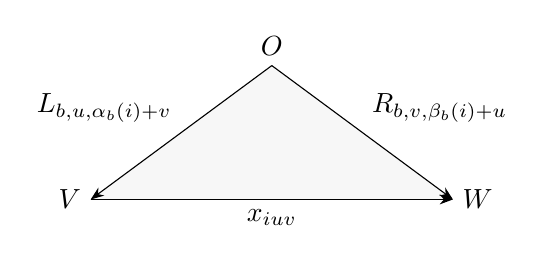
\begin{tikzpicture}[scale=1.0,>=Stealth]
 \coordinate (O) at (0,1.7);
 \coordinate (V) at (-2.3,0);
 \coordinate (W) at (2.3,0);
 \fill[black!3] (O)--(V)--(W)--cycle;
 \draw[->] (O)--node[above left] {$L_{b,u,\alpha_b(i)+v}$}(V);
 \draw[->] (O)--node[above right] {$R_{b,v,\beta_b(i)+u}$}(W);
 \draw[->] (V)--node[below] {$x_{iuv}$}(W);
 \node[above] at (O) {$O$};
 \node[left] at (V) {$V$};
 \node[right] at (W) {$W$};
\end{tikzpicture}
\caption{The incidence of the three oriented sides of one face.
The drawing is schematic; the metric face is the hyperbolic triangle
with angles \eqref{eq:angles}.}
\label{fig:triangle}
\end{figure}

Recall that the angular link at a vertex has a vertex for each
incident edge germ and an edge for each face corner, with length
equal to that corner's angle. A reduced path has no immediate edge
reversal. Reduction is also required at the closing seam of a
cyclically reduced closed path. Disconnected directions have infinite
link distance.

\begin{lemma}\label{lem:links}
Every nonempty cyclically reduced closed path in the link of $O$
has length at least $21\pi/10$. At $V$ and $W$ the corresponding
bound is $9\pi/4$. Moreover, at either $V$ or $W$, distinct
$x$-directions with the same label $i$ have link distance at least
$9\pi/4$, or lie in different components.
\end{lemma}

\begin{proof}
At $O$, a block contributes a complete bipartite graph between its
$L$- and $R$-directions. To see that it is simple, fix
$L_{b,u,j}$ and $R_{b,v,k}$. Their corner must use the unique label
with
\[
 \alpha_b(i)=j-v,\qquad \beta_b(i)=k-u.
\]
Directions belonging to different blocks are distinct. Thus the
whole link is a disjoint union of simple complete bipartite graphs.
Its nonempty reduced closed paths have at least four edges, with
length at least $4\theta_O=21\pi/10$.

Map the link at $V$ to the punctured incidence graph by sending
the direction $x_{iuv}$ to $i$ and the direction $L_{b,u,j}$ to
$p(b)$. Each corner maps to the corresponding incidence edge.
This is a graph immersion. At an $x_{iuv}$-direction, a specified
point $z$ allows at most one corner, since $i$ belongs to at most
one block at $z$. At an $L_{b,u,j}$-direction, a specified label
$i$ forces $v=j-\alpha_b(i)$ modulo $s_b$; there is at most one such
$v\in[r]$ because $s_b\ge r$. This proves local injectivity on
incident edges. The argument at $W$ is identical, using
$u=k-\beta_b(i)$ modulo $t_b$ and $t_b\ge r$.

An immersion preserves reduction, including reduction at a closing
seam. Every nonempty cyclically reduced closed link path therefore
maps to a reduced closed walk in the incidence graph. Such a walk
contains a cycle. By Lemma~\ref{lem:girth}, it has at least ten
edges, and its angular length is at least
$10\theta_V=9\pi/4$.

Finally, a reduced path between distinct $x$-directions with the
same label maps to a nonempty closed walk reduced at every internal
vertex. The closing seam need not be reduced. Nevertheless the
walk contains a simple cycle: a shortest positive subinterval with
equal endpoints cannot have length one in a simple graph, or length
two without an internal reversal. It is a simple cycle of length
at least ten. Applying this to a shortest link path proves the
distance assertion.
\end{proof}

\begin{proposition}\label{prop:cat}
The universal cover of $K$ is a proper $\CAT(-1)$ space. The group
$G=\pi_1(K,O)$ acts on it freely, properly and cocompactly by
isometries. It follows that $G$ is torsion-free and word-hyperbolic
and that $K$ is a finite two-dimensional $K(G,1)$.
\end{proposition}

\begin{proof}
All closed reduced link paths in Lemma~\ref{lem:links} have length
greater than $2\pi$. The metric link criterion therefore makes
$K$ locally $\CAT(-1)$; see
\cite[Theorem~II.5.2 and Lemma~II.5.6]{BH}.
There are finitely many shapes. The interiors of edges and faces
satisfy the same local curvature condition.

For a convention requiring intersections of cells to be single
faces, take a compatible geodesic barycentric subdivision. The
closed cells embed, so distinct cells provide distinct barycentric
vertices, even when there are parallel original edges. This produces
a genuine finite simplicial subdivision with the same metric. At a
new face-interior vertex the link is a circle of length $2\pi$;
at a new edge-interior vertex it is a union of length-$\pi$ paths
between the two edge directions. These also satisfy the link
criterion.

The lifted metric on the universal cover is complete. Cartan--Hadamard
\cite[Theorem~II.4.1]{BH} makes it $\CAT(-1)$. A cover of a finite
complex is locally finite, and with these finitely many positive
cell shapes the complete length metric is proper. Deck
transformations act freely and properly, and the quotient is the
compact complex $K$.

A finite group of isometries of a complete $\CAT(0)$ space fixes a
point \cite[Corollary~II.2.8]{BH}. A finite-order deck transformation
must therefore be the identity, so $G$ is torsion-free. A $\CAT(-1)$
space is Gromov-hyperbolic, and a proper cocompact isometric action
on this geodesic space identifies $G$, up to quasi-isometry, with
the universal cover \cite[Chapters~I.8 and~III.H]{BH}. Hence $G$
is word-hyperbolic. Finally, a $\CAT(-1)$ space is contractible,
which proves the classifying-space assertion.
\end{proof}

Choose a path $c_A$ from $O$ to each vertex $A$, with $c_O$ empty.
For an oriented edge $e:A\to B$, let $g_e$ be the class of
$c_A e c_B^{-1}$. We multiply loops in path order. Each face gives
\begin{equation}\label{eq:group-triangle}
 g_{L_{b,u,\alpha_b(i)+v}}\,g_{x_{iuv}}\,
                   g_{R_{b,v,\beta_b(i)+u}}^{-1}=1.
\end{equation}
Choosing the $c_A$ in a spanning tree gives the usual finite
presentation: the edge symbols, the triangular relators, and the
relations setting tree edges equal to the identity.

\begin{lemma}\label{lem:nontrivial}
Every element
\begin{equation}\label{eq:group-rectangle}
 w_{i;u,u',v,v'}=
 g_{x_{iuv}}g_{x_{iu'v}}^{-1}
 g_{x_{iu'v'}}g_{x_{iuv'}}^{-1},
 \qquad u\ne u',\quad v\ne v',
\end{equation}
is nonidentity in $G$.
\end{lemma}

\begin{proof}
After cancellation of the connecting paths, the word is conjugate
to the closed four-edge path
$x_{iuv}x_{iu'v}^{-1}x_{iu'v'}x_{iuv'}^{-1}$.
Every turn compares distinct $x$-directions with the same label.
Their link distance is greater than $\pi$ by
Lemma~\ref{lem:links}, so the path is a positive-length closed
local geodesic. If it were nullhomotopic, its lift to the universal
cover would be a positive-length closed local geodesic. In a
$\CAT(-1)$ space every local geodesic is a geodesic, which rules
this out \cite[Proposition~II.1.4]{BH}.
\end{proof}

\section{Excluding sofic approximations}\label{sec:sofic}

We use the usual finite-set definition of soficity
\cite{Pestov}. A group $H$ is sofic if, for every finite
$F\subset H$ containing $1$ and every $\eta>0$, there exist $D\ge1$
and a map $\phi:F\to\Sym(D)$ such that $\phi(1)=\id$,
\[
 d_H(\phi(a)\phi(b),\phi(ab))<\eta
 \quad(a,b,ab\in F),
\]
and $d_H(\phi(a),\id)>1-\eta$ for $a\in F\setminus\{1\}$.
This version includes asymptotic freeness as part of the definition.

We spell out the finite-word passage to keep the quantifiers clear.
Fix finitely many words in a finite alphabet of elements of $H$ and
their inverses. Include in $F$ the letters, their inverses, all word
prefixes, and $1$. If a nonempty word has length $\ell$ and has $k$ inverse
letters, evaluating it in the permutations assigned to the positive
letters differs from $\phi$ of its value by at most
$(\ell-1+k)\eta$. Indeed, each inverse substitution costs less than
$\eta$, by approximate multiplication of $a$ and $a^{-1}$, and
each prefix multiplication costs less than $\eta$.

\begin{proposition}\label{prop:no-sofic-target}
For the group $G$ constructed above, there is no homomorphism
$f:G\to H$ to a sofic group for which every rectangle
\eqref{eq:group-rectangle} has nonidentity image.
\end{proposition}

\begin{proof}
Suppose such an $f$ exists. Apply the finite-word observation in
$H$ to all the images of the triangular words and the rectangular
words, using the edge elements as the positive alphabet. There
are finitely many of each, with the incidence data already fixed.
Choose a sofic model of the resulting finite set and assign
$\phi(f(g_e))$ to every edge $e$.

Each triangular word has length three and one inverse letter.
Its group value is $1$ by \eqref{eq:group-triangle}, so its
Hamming defect is less than $3\eta$. A rectangular word has
length four and two inverse letters. Its evaluated permutation
is within $5\eta$ of $\phi(f(w))$. Since $f(w)\ne1$, the latter
has fixed-point proportion less than $\eta$. The fixed-point
proportion of the evaluated rectangle is therefore less than
$6\eta$. These estimates also cover edge elements that happen
to be the identity.

To obtain an explicit contradiction, set
\begin{equation}\label{eq:tolerance}
 \eps_0=\frac{1}{100rq}.
\end{equation}
Choose $\eta<\eps_0/6$. Then every triangle defect and every
rectangle fixed-point proportion is less than $\eps_0$.
Each retained line has exactly $q-1$ punctured incidences, so
$S_{\rm reg}\le N(q-1)$. Theorem~\ref{thm:rank} would imply
\begin{align*}
 \Delta
 &\le r^2\bigl(S_{\rm reg}+N/8\bigr)\eps_0\\
 &\le r^2Nq\eps_0
 =\frac{rN}{100}
 \le\frac{10^{-5}r}{100}\,m
 =\frac{3m}{25}.
\end{align*}
This contradicts $\Delta\ge m/5$ from
Proposition~\ref{prop:instance}.
\end{proof}

\begin{proof}[Proof of Theorem~\ref{thm:main}]
Proposition~\ref{prop:cat} gives all the geometric conclusions,
and Lemma~\ref{lem:nontrivial} shows that every rectangle is
nonidentity. If $G$ were sofic, its identity homomorphism would
contradict Proposition~\ref{prop:no-sofic-target}.

For the last assertion, let $\mathcal W$ be the finite set of
rectangle elements. Suppose that for every $w\in\mathcal W$ there
were a homomorphism $f_w:G\to H_w$ to a sofic group with
$f_w(w)\ne1$. The product map into $\prod_{w\in\mathcal W}H_w$
would preserve every rectangle. Finite products of sofic groups
are sofic: for a finite set in a product of $k$ factors and a
tolerance $\eta>0$, approximate its coordinate projections with
error less than $\eta/k$ and act on the Cartesian product of the
finite sets. Multiplication errors add at most, while fixed-point
proportions multiply; a nonidentity coordinate supplies freeness.
This
contradicts Proposition~\ref{prop:no-sofic-target}. Hence some
fixed $w\in\mathcal W$ is killed by all homomorphisms to sofic
groups, and $w\ne1$ by Lemma~\ref{lem:nontrivial}.
\end{proof}

The final argument identifies a finite set containing such a $w$;
it does not identify which rectangle has the universal kernel
property. This quantifier distinction is useful: for each target
there is a killed rectangle already by
Proposition~\ref{prop:no-sofic-target}, and closure under finite
products is what produces one rectangle working for all targets.

\section{Relation to the source construction and further scope}\label{sec:discussion}

The quantitative argument also applies directly to the original
family 252 incidence data. That source uses marked lines in
$\F_q^{20}$, a punctured incidence graph of girth at least fourteen,
the same two-block partitions, and the strict inequality
$Nr/4>2m+r|E|$. Its interpolation matrices satisfy
\eqref{eq:certificate}. Theorem~\ref{thm:rank} therefore applies
without any change in the combinatorial presentation. One may
replace its Euclidean face metric by the common hyperbolic shape
\eqref{eq:angles}; girth fourteen is more than sufficient for
Lemma~\ref{lem:links}. Thus every instance satisfying the stated
source hypotheses has the same obstruction to soficity. The
five-dimensional construction gives a different, smaller input to
the same mechanism.

This also explains precisely where the passage beyond residual
finiteness occurs. In \cite{OA252}, nontrivial rectangles act without
fixed points in a regular representation of a finite quotient.
Here their traces may be positive, and the triangular factorizations
may fail. Lemmas~\ref{lem:rectangle-rank} and
\ref{lem:triangle-rank} measure both losses. The tensor identity
does not require modification. The advertised formalization scope
of family 252 is its non-residual-finiteness theorem
\cite{OA252formal}; it does not certify the approximate-permutation
extension proved here.

For comparison with the literature, OpenAI's earlier construction
\cite[Chapter~3]{OA197} gives a nonsofic group through a
property-$(T)$ and expander mechanism. Fournier-Facio
\cite[Theorem~1.3]{FF} gives a finitely presented torsion-free
nonsofic group, and Kun--Thom \cite[Theorem~A]{KT} give
nonsofic generalized wreath products and doubles. Their discussion
of a hyperbolic group admitting a nonsofic probability-measure-
preserving action is a different assertion from nonsoficity of the
group itself. The conditional hyperbolic construction of
Chapman--Peled \cite{CP} uses permutation cocycle stability in a
random complex. The rank estimate here instead acts directly on
the approximate data. None of these comparisons is needed as an
input to the proof.

The size reduction does not make the numerical construction small.
For the parameters of Proposition~\ref{prop:instance}, $m=q^5$ has 92 decimal digits,
$N=\lfloor q/10\rfloor^5$ has 87, and the bound
$r^2N(q-1)$ for the number of triangles has 118. An affine map $U$
has only thirty field coefficients, but the present acceptance
test evaluates a huge incidence ledger. A short symbolic
certificate for a particular admissible $U$ would make the
construction easier to inspect. Existence of an admissible $U$,
however, follows from the finite counting argument above and does
not depend on actually running that search.

The obstruction is specific to permutations. It gives no
nonhyperlinearity conclusion: a unitary matrix $e^{it}I_D$ can
approach $I_D$ in normalized Hilbert--Schmidt norm while their
difference has rank $D$. Nor does rectangle separation in normalized
rank replace Lemma~\ref{lem:rectangle-rank} for arbitrary
invertible matrices. For distinct positive real numbers $a_u,b_v$,
the blocks $X_{uv}=(a_u+b_v)I_D$ form a matrix of rank $2D$, while
every nondegenerate rectangle differs from the identity by a
full-rank matrix. Thus neither nonhyperlinearity nor failure of
linear soficity is established by the present argument.
No property-$(T)$ conclusion is asserted for $G$.

\subsection*{Disclosure}
The mathematical derivation and manuscript were produced with
substantial assistance from OpenAI language models. The manuscript
is released as a candidate proof for independent mathematical
scrutiny and has not undergone external peer review. The human
contact listed above has not independently certified every argument.
The approximate-permutation extension and the five-dimensional
construction have not been formally verified.

\begin{thebibliography}{99}

\bibitem{BH}
M. R. Bridson and A. Haefliger,
\emph{Metric Spaces of Non-Positive Curvature},
Grundlehren der mathematischen Wissenschaften, vol.~319,
Springer-Verlag, Berlin, 1999.
\href{https://doi.org/10.1007/978-3-662-12494-9}{doi:10.1007/978-3-662-12494-9}.

\bibitem{CP}
M. Chapman and Y. Peled,
\emph{Cocycle stability in permutations of random simplicial complexes},
preprint, 2025, version~2.
\href{https://arxiv.org/abs/2509.21566v2}{arXiv:2509.21566v2}.

\bibitem{FF}
F. Fournier-Facio,
\emph{A torsion-free non-sofic group},
preprint, 2026, version~2.
\href{https://arxiv.org/abs/2608.02025v2}{arXiv:2608.02025v2}.

\bibitem{KT}
G. Kun and A. Thom,
\emph{Nonsofic wreath products of residually finite groups},
preprint, 2026, version~3.
\href{https://arxiv.org/abs/2608.06222v3}{arXiv:2608.06222v3}.

\bibitem{LUW}
F. Lazebnik, V. A. Ustimenko and A. J. Woldar,
\emph{A new series of dense graphs of high girth},
Bull. Amer. Math. Soc. (N.S.) \textbf{32} (1995), 73--79.
\href{https://arxiv.org/abs/math/9501231}{arXiv:math/9501231}.

\bibitem{OA252}
OpenAI,
\emph{A torsion-free hyperbolic group that is not residually finite},
family 252, manuscript dated 23 September 2026, in the
\texttt{openai/math} source collection.
\href{https://github.com/openai/math/blob/adc7f1241b42e322a6451854ab7e4b4c146bf78a/preprints/a-torsion-free-hyperbolic-group-that-is-not-residually-finite-September-23-2026/build/paper.tex}{Pinned manuscript source};
\href{https://github.com/openai/math/blob/adc7f1241b42e322a6451854ab7e4b4c146bf78a/preprints/a-torsion-free-hyperbolic-group-that-is-not-residually-finite-September-23-2026/build/sections/construction.tex}{construction and rank argument}.
Repository revision \texttt{adc7f1241b42e322a6451854ab7e4b4c146bf78a}.

\bibitem{OA252formal}
OpenAI,
\emph{Scope of the Lean formalization for family 252}, 2026.
\href{https://github.com/openai/math/blob/adc7f1241b42e322a6451854ab7e4b4c146bf78a/lean/docs/252.md}{\texttt{lean/docs/252.md}},
at the same revision as \cite{OA252}.

\bibitem{OA197}
OpenAI,
\emph{Nonsofic groups exist},
Chapter~3 of \emph{Ten Advances in Mathematics and Theoretical
Computer Science}, updated 6 August 2026.
\href{https://cdn.openai.com/pdf/ten-proofs-oai.pdf}{Online manuscript}.

\bibitem{Pestov}
V. G. Pestov,
\emph{Hyperlinear and sofic groups: a brief guide},
Bull. Symbolic Logic \textbf{14} (2008), no.~4, 449--480.
\href{https://arxiv.org/abs/0804.3968}{arXiv:0804.3968}.

\end{thebibliography}
\end{document}
